% APNs packed (apns-pack-v1) encoding: message, field header byte, worked example (single column).
% Build: pdflatex fig_packed.tex.  Coordinates in mm, y increasing DOWNWARDS.
\documentclass[tikz,border=2pt]{standalone}
\usepackage[scaled]{helvet}
\renewcommand{\familydefault}{\sfdefault}
\usepackage[T1]{fontenc}
\usetikzlibrary{arrows.meta}

\definecolor{cTealF}{HTML}{DDF1EE}   \definecolor{cTealS}{HTML}{1D8C7B}
\definecolor{cBlueF}{HTML}{DCEAF9}   \definecolor{cBlueS}{HTML}{2F6DB5}
\definecolor{cAmbF}{HTML}{FBEBCB}    \definecolor{cAmbS}{HTML}{B8781A}
\definecolor{cGrayF}{HTML}{F1F1EF}   \definecolor{cGrayS}{HTML}{8A8A85}

% \fld{x}{y}{w}{fill}{stroke}{text}: one field box, 6 mm high
\newcommand{\fld}[6]{\draw[fill=#4,draw=#5,line width=0.4pt] (#1,#2) rectangle ++(#3,6);
  \node[font=\scriptsize,inner sep=0pt,align=center] at (#1+#3/2,#2+3) {#6};}
\newcommand{\fcap}[3]{\node[font=\tiny,inner sep=0pt,align=center,text=black!70] at (#1,#2) {#3};}
\newcommand{\ttl}[3]{\node[font=\scriptsize\bfseries,inner sep=0pt,anchor=west] at (#1,#2) {#3};}

\begin{document}
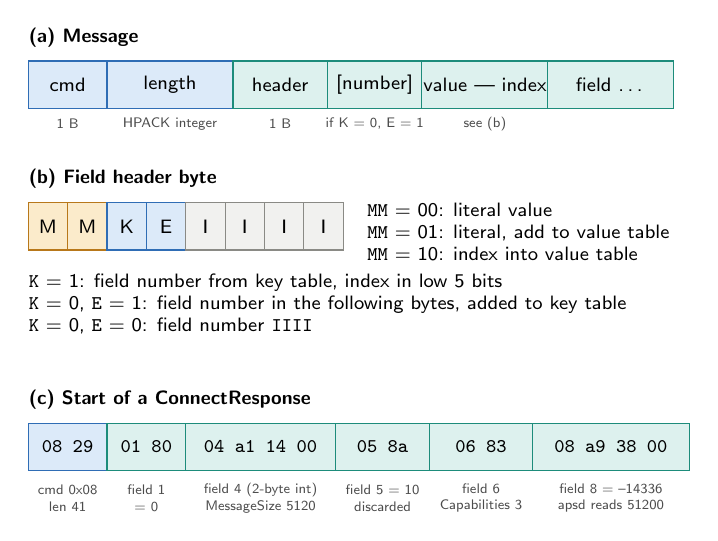
\begin{tikzpicture}[x=1mm,y=-1mm]
% ---- (a) message ---------------------------------------------------------
\ttl{0}{18}{(a) Message}
\fld{0}{21}{10}{cBlueF}{cBlueS}{cmd}
\fld{10}{21}{16}{cBlueF}{cBlueS}{length}
\fld{26}{21}{12}{cTealF}{cTealS}{header}
\fld{38}{21}{12}{cTealF}{cTealS}{[number]}
\fld{50}{21}{16}{cTealF}{cTealS}{value | index}
\fld{66}{21}{16}{cTealF}{cTealS}{field \dots}
\fcap{5}{29}{1 B}  \fcap{18}{29}{HPACK integer}  \fcap{32}{29}{1 B}  \fcap{44}{29}{if K = 0, E = 1}  \fcap{58}{29}{see (b)}

% ---- (b) field header byte -----------------------------------------------------
\ttl{0}{36}{(b) Field header byte}
\foreach \i/\b/\f/\s in {0/M/cAmbF/cAmbS,1/M/cAmbF/cAmbS,2/K/cBlueF/cBlueS,3/E/cBlueF/cBlueS,4/I/cGrayF/cGrayS,5/I/cGrayF/cGrayS,6/I/cGrayF/cGrayS,7/I/cGrayF/cGrayS}
  { \fld{\i*5}{39}{5}{\f}{\s}{\b} }
\node[font=\scriptsize,anchor=north west,align=left,inner sep=0pt] at (43,39) {%
\texttt{MM} = 00: literal value\\
\texttt{MM} = 01: literal, add to value table\\
\texttt{MM} = 10: index into value table};
\node[font=\scriptsize,anchor=north west,align=left,inner sep=0pt] at (0,48) {%
\texttt{K} = 1: field number from key table, index in low 5 bits\\
\texttt{K} = 0, \texttt{E} = 1: field number in the following bytes, added to key table\\
\texttt{K} = 0, \texttt{E} = 0: field number \texttt{IIII}};

% ---- (c) worked example ----------------------------------------------------------------
\ttl{0}{64}{(c) Start of a ConnectResponse}
\foreach \x/\w/\t/\f/\s in {0/10/08 29/cBlueF/cBlueS, 10/10/01 80/cTealF/cTealS, 20/19/04 a1 14 00/cTealF/cTealS,
                           39/12/05 8a/cTealF/cTealS, 51/13/06 83/cTealF/cTealS, 64/20/08 a9 38 00/cTealF/cTealS}
  { \draw[fill=\f,draw=\s,line width=0.4pt] (\x,67) rectangle ++(\w,6);
    \node[font=\scriptsize\ttfamily,inner sep=0pt] at (\x+\w/2,70) {\t}; }
\fcap{5}{76.5}{cmd 0x08\\len 41}
\fcap{15}{76.5}{field 1\\= 0}
\fcap{29.5}{76.5}{field 4 (2-byte int)\\MessageSize 5120}
\fcap{45}{76.5}{field 5 = 10\\discarded}
\fcap{57.5}{76.5}{field 6\\Capabilities 3}
\fcap{74}{76.5}{field 8 = \textendash 14336\\apsd reads 51200}
\end{tikzpicture}
\end{document}
